% -- TUTORIAL REFS+LABEL --
% Il goal \ref{goal:info} si trova a pagina \pageref{goal:info}
% -- END TUTORIAL --

% --- TUTORIAL SCENARIOS --- 
% \scenario{etichetta}{titolo}{testo}
% --- END TUTORIAL ---

\pagebreak
\subsection{Scenarios}
\scenario{michael}{A shy student}{Michael does not want to lose his favorite class, but unfortunately a strike has been announced for today. Since he lives not too far nor too near from his university, he decides to take a taxi; unfortunately, his shyness does not let him call for one. So he decides to use MyTaxiService, the application developed by his own city, in order to get a cab as soon as possible. As a registered user, the only thing he has to do is open the app, log in, click on the “Get a taxi now” button and just wait for the response to come.}

\scenario{siegfried}{The german IT entrepreneur}{Siegfried is a German IT entrepreneur who has just arrived to the city for a working meeting. Since he does not trust the public transport service, he wants to rely on the taxi service. After a quick search on Google, he finds myTaxiService and decides to download the app. After filling in his own personal data, including the cell phone number, he clicks on the Submit button; after few seconds, he receives an email with a link so that he can confirm his registration and start using the service.}
%(SMS??)

\scenario{norma}{Taxi reservation}{Norma has to fly to Denmark the next day early in the morning. Due to this, she cannot take any public transportation service. Being a very organized woman, she decides to reserve a taxi the night before. Since she has very little time, she wants a friendly and fast way to do so; she decides then to use the “Reseve a taxi” functionality provided by myTaxiService web app on her laptop. The only things she has to insert are her starting point, her destination and when to leave. After that, a confirmation message is given and a taxi is successfully reserved.}

\scenario{riccardo}{The amusement park lover}{Riccardo loves amusement parks and so he decides to organize a full day in the nearest one. He knows that the trains and busses will be pretty unusable; since he wants to spend as much as possible on his entertainment, he decides to reserve a taxi the night before by using the Sharing option. Luke and Christine decide to do the same too and find out that Riccardo had already reserved a vehicle for the same date and the same starting point. They accept to take the same taxi and equally divide the fees.}

\scenario{max}{The taxi driver}{Max is a driver working for the public taxi service of his own city. During his daytime turn, his wife Marilyn calls from the city hospital saying that she is about to give birth to their child. During his frenetic race to the hospital a request comes from the system, but Max refuses to accept it by clicking on the “Decline Request” button. The system puts the driver in his zone queue tail. After that, Max realizes that he will be busy for a while so he decides to change his status to ``unavailable".}

\scenario{matthew}{Cancel a reservation}{Matthew is an engineering student who wanted to surprise his girlfriend, so he decided to reserve a taxi planning to show up in front of her house with a bouquet of roses. Unfortunately, few hours before the big event, her girlfriend broke up with him using a text message. With his heart broken, Matthew thinks that showing up at her place wouldn't be a good idea so he decides to go through his app in the ``manage reservations'' section and cancel his reservation for that day.}

% --- TUTORIAL USECASE --- 
% \usecase{Name}{Description}{PrimaryActor}{BasicFlow}{AlternateFlow}
% --- END TUTORIAL ---
\pagebreak
\subsection{Use cases and UML diagrams}
\vfill
\includegraphics[scale=0.5]{UseCase.png}
\pagebreak
% ---------- SIGN UP --------------------
\usecase
{Sign Up}
{Registration to the system by a customer-to-be.}
{Guest}
{
\begin{enumerate}
	\item Guests visit the service home page
	\item The guest clicks on ``Register''
	\item The system outputs the form on screen
	\item The guest inserts his name, mail, password and mobile phone number and then clicks on ``Continue''
	\item The system checks if the mail, password and phone number are syntactically valid; if so, it sends a mail and a sms with a verification link
	\item The guest clicks on the link and verifies his account by inserting the code sent by sms
	\item The guest is now a customer registered to the service
\end{enumerate}
}
{
/
}
{ 
\begin{enumerate}
	\item The guest is already registered
	\item One or more fields are not well-formed
	\item Username already in use
    \item The validation link is not more valid (after 48 hours)
\end{enumerate}
}

% SEQUENCE 
\sequence{SignUp}{Sign Up}

% ---------- SIGN IN --------------------
\usecase
{Sign in}
{Login by a customer}
{Guest, Customer}
{
\begin{enumerate}
	\item A guest visits the service home page
	\item The guest clicks on ``Log in''
	\item The system outputs the form on screen
	\item The guest inserts his name, password then clicks on ``Continue''
	\item The system checks if the mail, password and phone number are valid and present in the DB
	\item The guest is redirected to the home page and recognized as a customer from now on.
\end{enumerate}
}
{
/
}
{ \begin{enumerate}
	\item The user and/or password are incorrect
	\item One or more fields are not well-formed
	\item Username not registered
\end{enumerate} }

% SEQUENCE 
\sequence{SignIn}{Sign In}

% ---------- RESERVATION --------------------
\usecase
{Reserve a taxi}
{Reservation of a taxi by a customer for a specified date, start and destination}
{Customer}
{
\begin{enumerate}
	\item The customer clicks on ``Reserve a taxi''
	\item The system shows the reservation page
	\item The customer fills in the mandatory information (starting point, destination, payment method, number of people and date-time)
	\item The system registers the request and inserts it in the correct zone queue, according to the specified starting point.
	\item The customer is informed that the operation did not fail thanks to a confirmation screen
	\item TaxiHandler will evaluate it when needed (see ``Allocate a taxi'' use case)
\end{enumerate}
}
{
\textbf{Sharing option}
\begin{enumerate}
	\item Same operations as before till point 3
	\item The user also specifies that he wants to share his taxi
	\item The TaxiHandler assigns the customer to the first reserved taxi for that ride if present
	\item If there are no available shared rides, a new one is created on the spot
	\item Same operation as before from point 4 on
\end{enumerate}
}
{ 
\begin{itemize}
	\item The date and/or places are not valid
\end{itemize}
}

% SEQUENCE 
\sequence{Reservation}{Reservation}
\FSM{ReserveFlow}{Reserve FSM}

% ---------- REQUEST --------------------
\usecase
{Request a taxi}
{Quick taxi request for a customer who needs a taxi for the immediate future at its location}
{Customer, TaxiHandler}
{
\begin{enumerate}
	\item The customer clicks on ``Request a taxi''
	\item The customer fills in the mandatory information (starting point, destination, payment method and number of people)
	\item The system registers the request and inserts it in the correct zone queue, according to the specified starting point.
	\item TaxiHandler processes the call (see ``Allocate a taxi'' use case)
	\item The customer is informed that the operation did not fail thanks to a confirmation screen
\end{enumerate}
}
{
/
}
{ 
/
}

% SEQUENCE 
\pagebreak
\sequence{RequestTaxi}{Request a taxi}

% ---------- ALLOCATE --------------------
\usecase
{Delete reservation}
{Possibility of a customer to view and eventually delete one or more reservations made by him}
{Customer, Taxi Handler}
{
\begin{enumerate}
	\item The customer clicks on ``Manage reservations''.
	\item The customer sees the entire list of his reservations (with details for each one) and may delete them.
\end{enumerate}
}
{
/
}
{ 
\begin{itemize}
	\item The deleted reservation occurs in less than 10 minutes from the delete action.
\end{itemize}
}

% SEQUENCE 
\pagebreak
\sequence{DeleteReservation}{Delete a reservation}
\pagebreak
% ---------- ALLOCATE --------------------
\usecase
{Allocate a taxi}
{Selection and notification of a taxi driver to process a request or a reservation by the TaxiHandler}
{Taxi Handler, Taxi Driver}
{
\begin{enumerate}
	\item The TaxiHandler sends a notification to the first taxi driver who meets the requirements in the given zone queue.
	\item If a positive answer is given in 30 seconds the TaxiHandler provides to set the Driver as ``busy''.
	\item Otherwise the driver is moved to the bottom of the queue. TaxiHandler restarts the seek from step 1.
\end{enumerate}
}
{
/
}
{ 
/
}

% SEQUENCE 
\pagebreak
\sequence{AllocateTaxi}{Allocate a taxi}
\FSM{TaxiFSM}{Taxi FSM}

% WORKFLOW 
\pagebreak
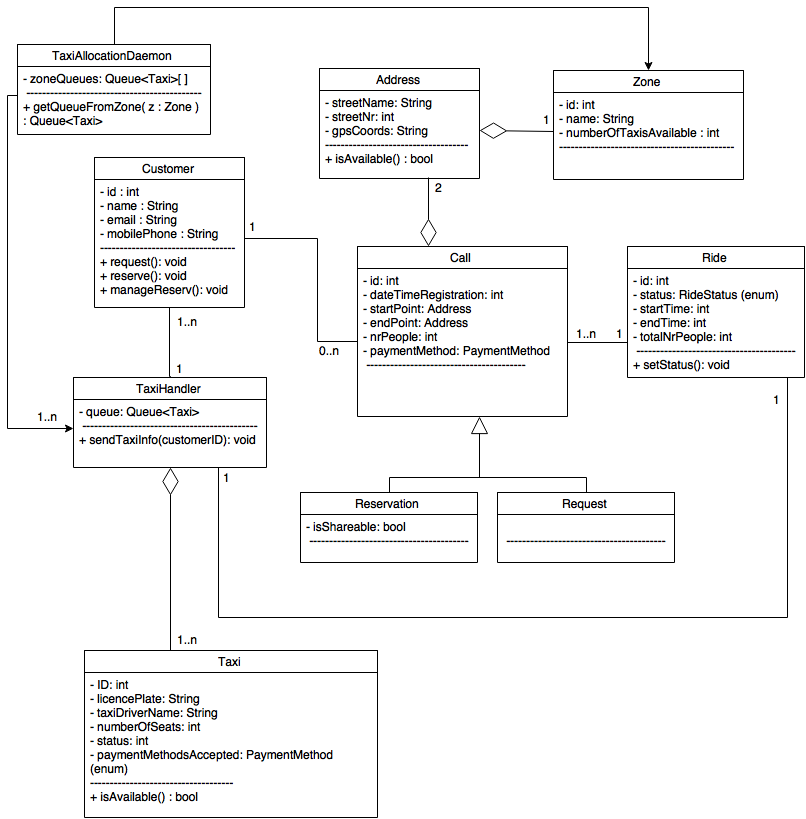
\includegraphics[scale=0.5]{ClassDiagram.png}
